\hypertarget{TreeGrow_8c}{
\section{TreeGrow.c File Reference}
\label{TreeGrow_8c}\index{TreeGrow.c@{TreeGrow.c}}
}
{\tt \#include \char`\"{}party.h\char`\"{}}\par


Include dependency graph for TreeGrow.c:\nopagebreak
\begin{figure}[H]
\begin{center}
\leavevmode
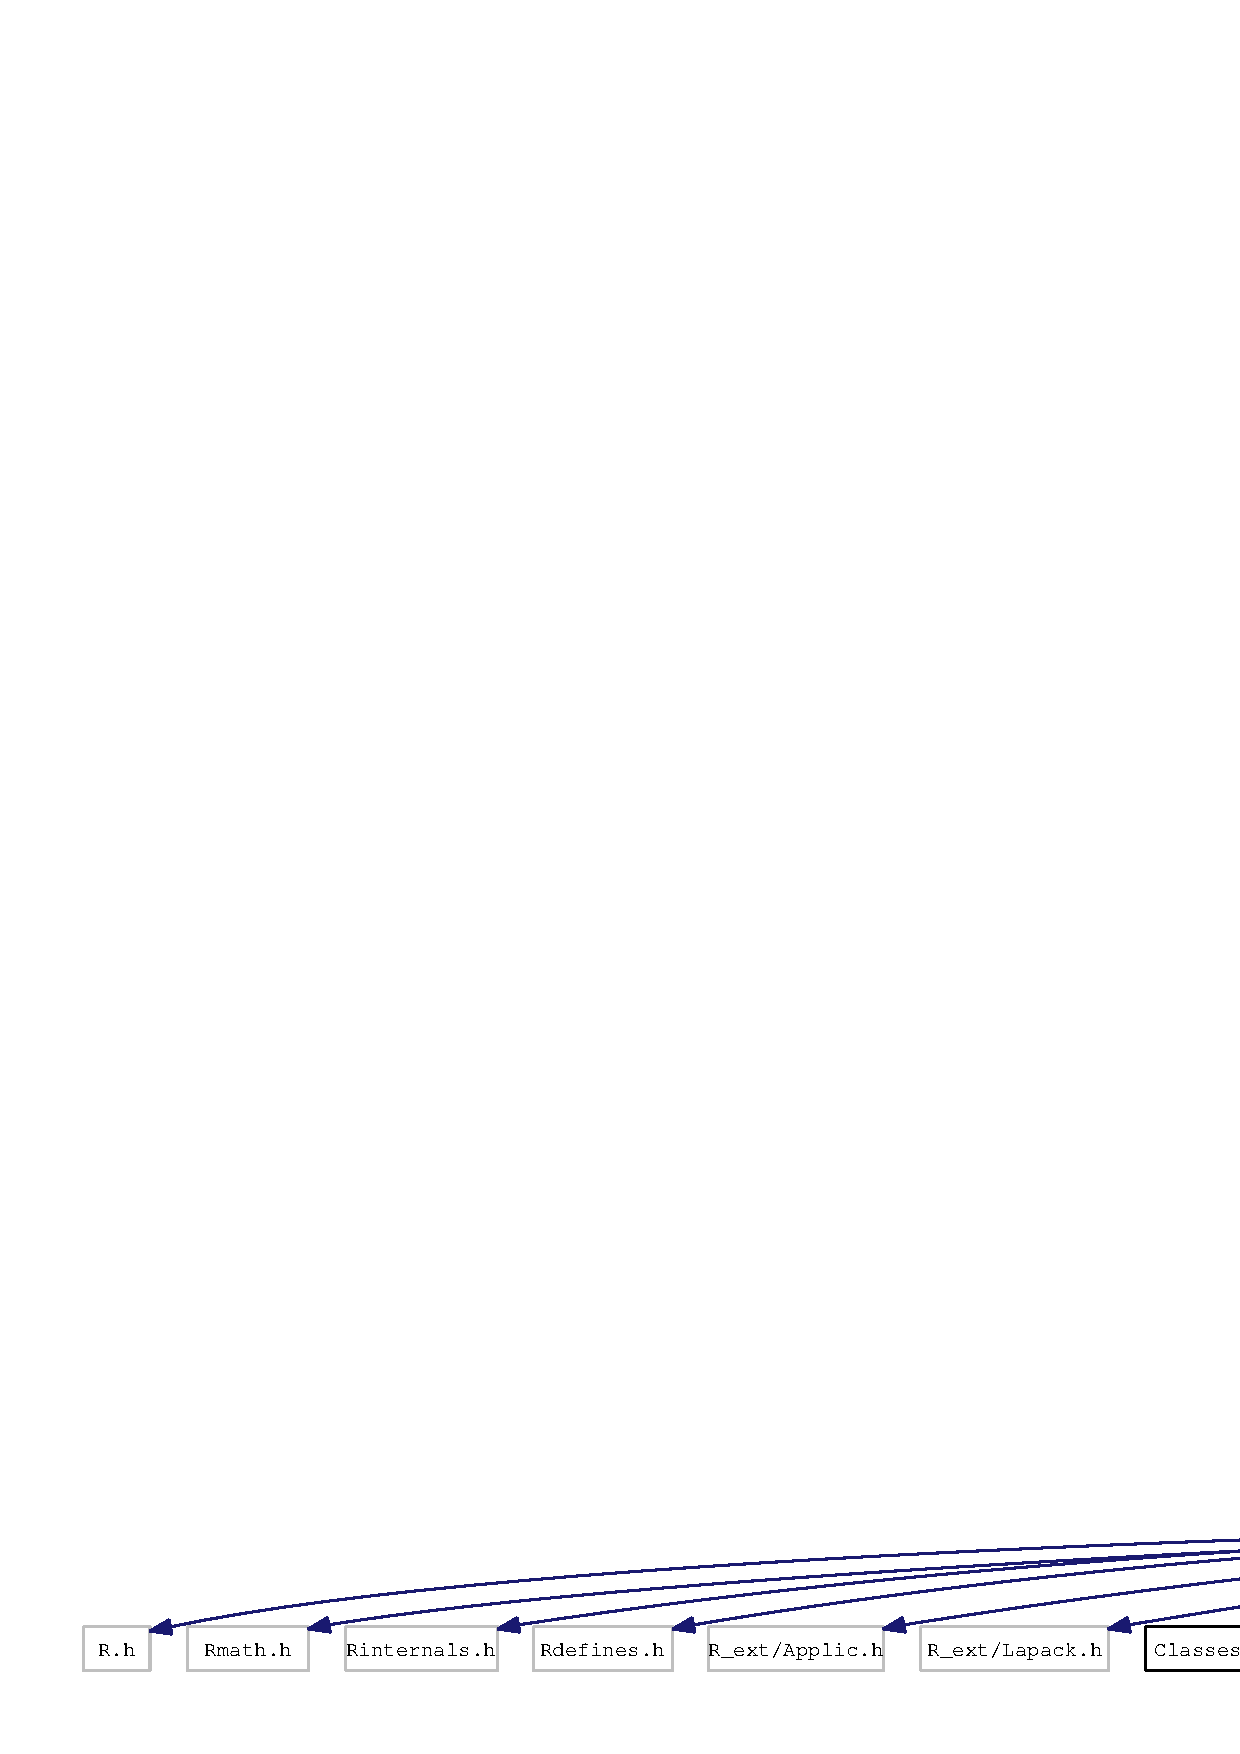
\includegraphics[width=420pt]{TreeGrow_8c__incl}
\end{center}
\end{figure}
\subsection*{Functions}
\begin{CompactItemize}
\item 
void \hyperlink{TreeGrow_8c_67d352c38f59d30c7b9954bf5d3a57ad}{C\_\-TreeGrow} (SEXP node, SEXP learnsample, SEXP fitmem, SEXP controls, int $\ast$where, int $\ast$nodenum, int depth)
\item 
SEXP \hyperlink{TreeGrow_8c_f9fe6e74563480c8eb5e4332fe9bca22}{R\_\-TreeGrow} (SEXP learnsample, SEXP weights, SEXP fitmem, SEXP controls, SEXP where)
\end{CompactItemize}


\subsection{Detailed Description}
The tree growing recursion

\begin{Desc}
\item[Author:]\end{Desc}
\begin{Desc}
\item[Author]hothorn \end{Desc}
\begin{Desc}
\item[Date:]\end{Desc}
\begin{Desc}
\item[Date]2007-07-23 09:44:00 +0200 (Mon, 23 Jul 2007) \end{Desc}


Definition in file \hyperlink{TreeGrow_8c-source}{TreeGrow.c}.

\subsection{Function Documentation}
\hypertarget{TreeGrow_8c_67d352c38f59d30c7b9954bf5d3a57ad}{
\index{TreeGrow.c@{TreeGrow.c}!C\_\-TreeGrow@{C\_\-TreeGrow}}
\index{C\_\-TreeGrow@{C\_\-TreeGrow}!TreeGrow.c@{TreeGrow.c}}
\subsubsection{\setlength{\rightskip}{0pt plus 5cm}void C\_\-TreeGrow (SEXP {\em node}, \/  SEXP {\em learnsample}, \/  SEXP {\em fitmem}, \/  SEXP {\em controls}, \/  int $\ast$ {\em where}, \/  int $\ast$ {\em nodenum}, \/  int {\em depth})}}
\label{TreeGrow_8c_67d352c38f59d30c7b9954bf5d3a57ad}


The main tree growing function, handles the recursion. \par
 \begin{Desc}
\item[Parameters:]
\begin{description}
\item[{\em node}]a list representing the current node \item[{\em learnsample}]an object of class `LearningSample' \item[{\em fitmem}]an object of class `TreeFitMemory' \item[{\em controls}]an object of class `TreeControl' \item[{\em where}]a pointer to an integer vector of n-elements \item[{\em nodenum}]a pointer to a integer vector of length 1 \item[{\em depth}]an integer giving the depth of the current node \end{description}
\end{Desc}


Definition at line 23 of file TreeGrow.c.

References C\_\-Node(), C\_\-splitnode(), C\_\-splitsurrogate(), C\_\-surrogates(), C\_\-TreeGrow(), check\_\-depth(), get\_\-maxsurrogate(), get\_\-nobs(), get\_\-splitctrl(), get\_\-stump(), get\_\-tgctrl(), S3get\_\-leftnode(), S3get\_\-nodeterminal(), S3get\_\-nodeweights(), S3get\_\-rightnode(), and S3set\_\-nodeID().

Referenced by C\_\-TreeGrow(), R\_\-Ensemble(), and R\_\-TreeGrow().

Here is the call graph for this function:\nopagebreak
\begin{figure}[H]
\begin{center}
\leavevmode
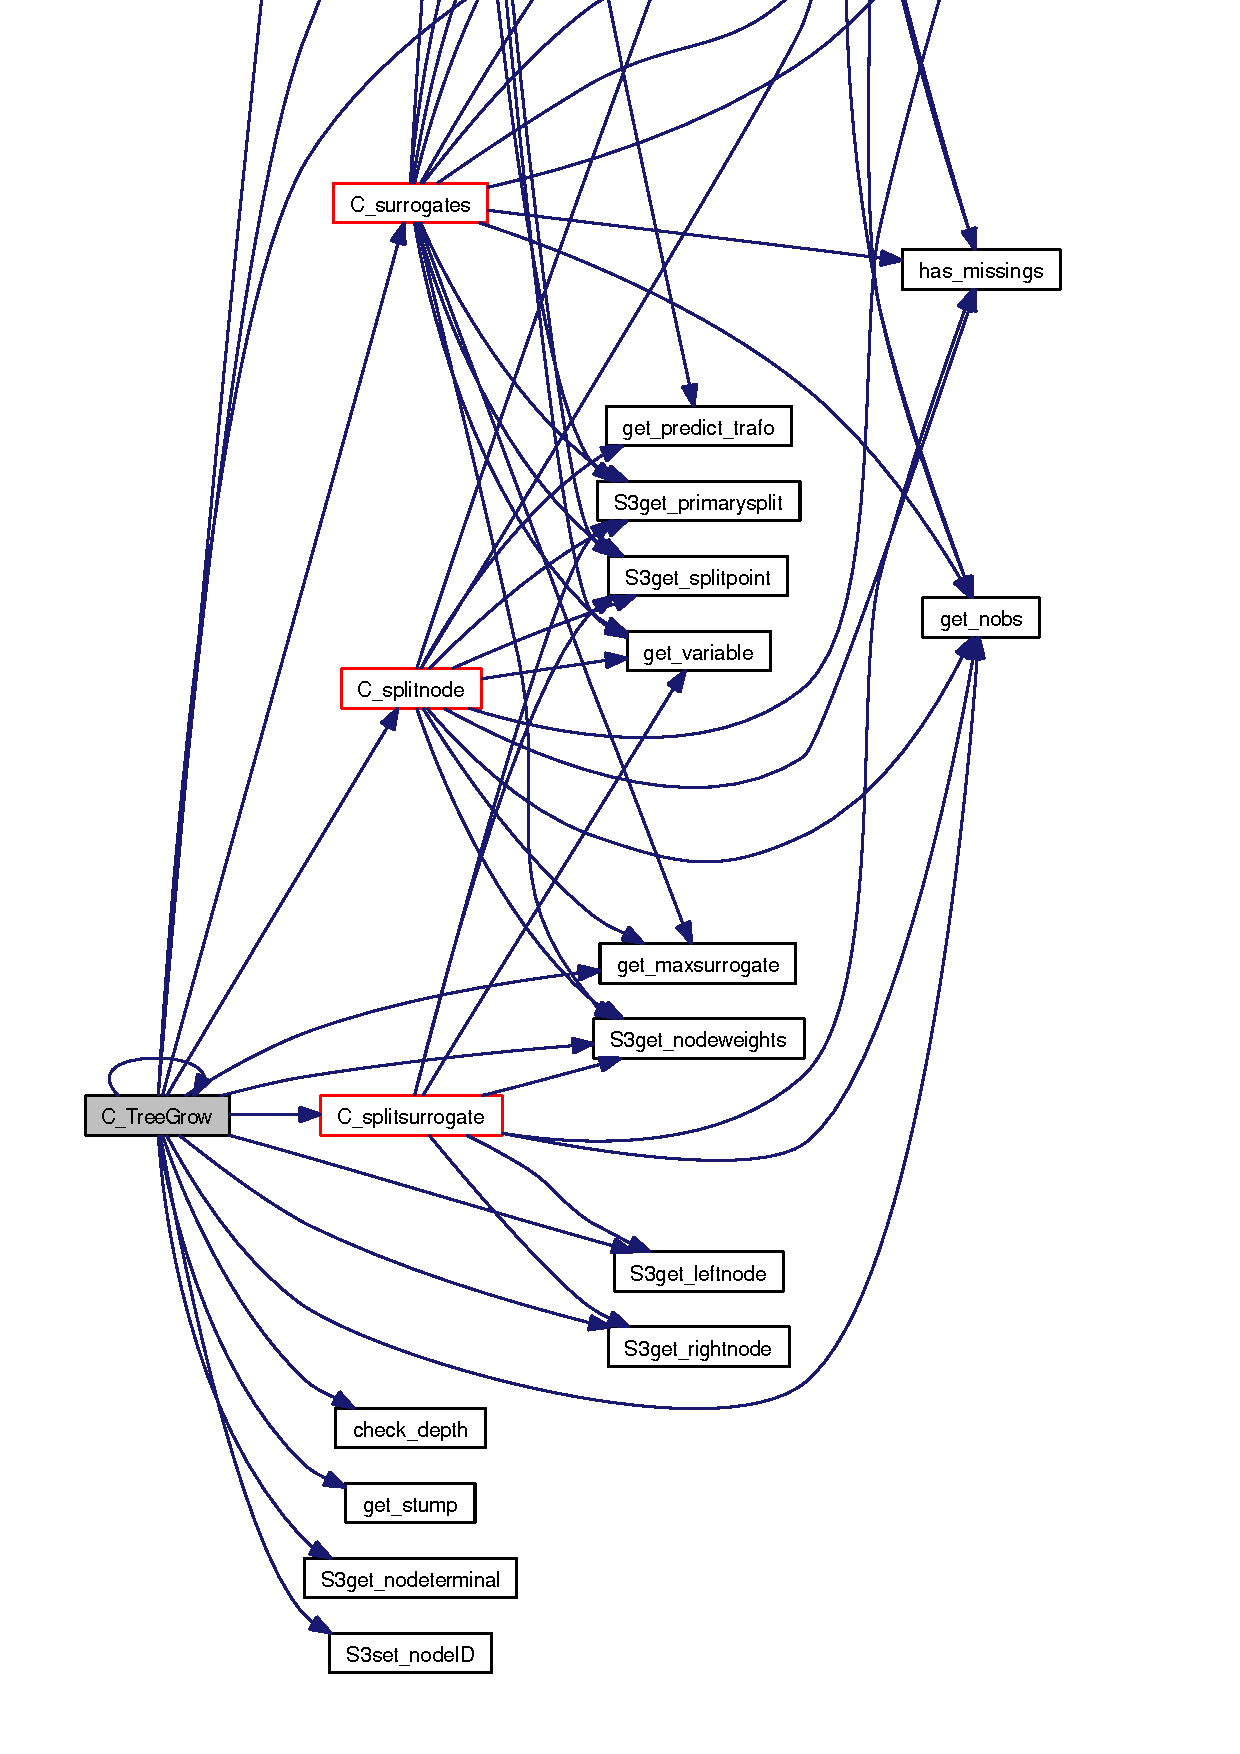
\includegraphics[width=303pt]{TreeGrow_8c_67d352c38f59d30c7b9954bf5d3a57ad_cgraph}
\end{center}
\end{figure}
\hypertarget{TreeGrow_8c_f9fe6e74563480c8eb5e4332fe9bca22}{
\index{TreeGrow.c@{TreeGrow.c}!R\_\-TreeGrow@{R\_\-TreeGrow}}
\index{R\_\-TreeGrow@{R\_\-TreeGrow}!TreeGrow.c@{TreeGrow.c}}
\subsubsection{\setlength{\rightskip}{0pt plus 5cm}SEXP R\_\-TreeGrow (SEXP {\em learnsample}, \/  SEXP {\em weights}, \/  SEXP {\em fitmem}, \/  SEXP {\em controls}, \/  SEXP {\em where})}}
\label{TreeGrow_8c_f9fe6e74563480c8eb5e4332fe9bca22}


R-interface to C\_\-TreeGrow\par
 \begin{Desc}
\item[Parameters:]
\begin{description}
\item[{\em learnsample}]an object of class `LearningSample' \item[{\em weights}]a vector of case weights \item[{\em fitmem}]an object of class `TreeFitMemory' \item[{\em controls}]an object of class `TreeControl' \item[{\em where}]a vector of node indices for each observation \end{description}
\end{Desc}


Definition at line 81 of file TreeGrow.c.

References C\_\-init\_\-node(), C\_\-TreeGrow(), get\_\-maxsurrogate(), get\_\-ninputs(), get\_\-nobs(), get\_\-predict\_\-trafo(), get\_\-splitctrl(), ncol(), NODE\_\-LENGTH, PL2\_\-responsesSym, and S3get\_\-nodeweights().

Here is the call graph for this function:\nopagebreak
\begin{figure}[H]
\begin{center}
\leavevmode
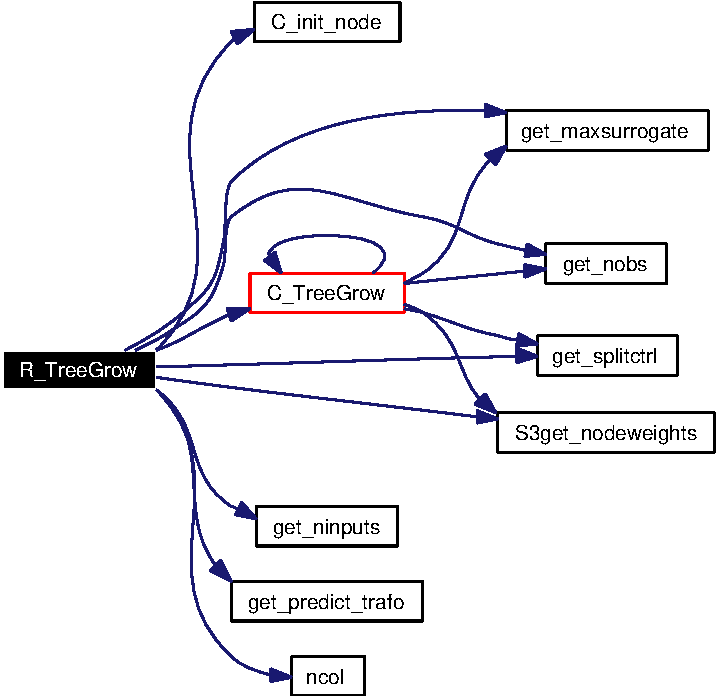
\includegraphics[width=356pt]{TreeGrow_8c_f9fe6e74563480c8eb5e4332fe9bca22_cgraph}
\end{center}
\end{figure}
